\documentclass[11pt, a4paper]{article}

\usepackage{xcolor}

\usepackage{parskip,setspace}
\usepackage{amsmath}
\usepackage{amssymb}
\usepackage{amsthm}
\usepackage[hmargin=2cm,vmargin=3cm]{geometry}

\newtheorem{Theorem}{Theorem}
\newtheorem{Proposition}[Theorem]{Proposition}
\newtheorem{Corollary}[Theorem]{Corollary}
\newtheorem{Comment}[Theorem]{Comment}
\newtheorem{Fact}[Theorem]{Fact}
\newtheorem{Lemma}[Theorem]{Lemma}
\theoremstyle{definition}
\newtheorem{Definition}[Theorem]{Definition}
\newtheorem{Example}[Theorem]{Example}

\usepackage{tikz}


\newtheorem{theorem}[Theorem]{Theorem}
\newtheorem{lemma}[Theorem]{Lemma}

\setlength{\itemsep}{0pt}
\setlength{\topsep}{0pt}
\setlength{\parindent}{0pt}
\setlength{\parskip}{6pt}

\newcommand{\bra}[1]{\left< #1 \right|}
\newcommand{\ket}[1]{\left| #1 \right>}

\newcommand{\iprod}[2]{\langle #1 | #2 \rangle}
\newcommand{\mprod}[3]{\langle #1 | #2 | #3 \rangle}
\newcommand{\oprod}[2]{| #1 \rangle\langle #2 |}

\newcommand{\proj}[3]{\begin{smallmatrix} #1 & #2 & #3 \end{smallmatrix}}
\newcommand{\projbf}[3]{\begin{smallmatrix} \mathbf{#1} & \mathbf{#2} & \mathbf{#3} \end{smallmatrix}}

\sloppy

\newcommand{\seq}[1]{\mathbf{#1}}
\newcommand{\floor}[1]{\left\lfloor #1 \right\rfloor}
\newcommand{\ceil}[1]{\left\lceil #1 \right\rceil}
\newcommand{\m}[1]{\tilde{#1}}
\parskip .7em                   %vskip between paragraphs

\title{Kochen-Specker Theorem Revisited and Strong Incomputability of Quantum Randomness}
\author{Alastair A. Abbott, Cristian S. Calude, Jonathan Conder and Karl Svozil}
\date{\today}

\begin{document}


\maketitle

\section{Definitions}% and Relevant Results}

\subsection{Notation}

We denote the set of natural numbers (in which we include 0) by $\mathbb{N}=\{0,1,2,\dots\}$, the positive integers by $\mathbb{N}^+=\mathbb{N}\setminus\{0\}$, and the set of complex numbers by $\mathbb{C}$.
We use the standard quantum mechanical bra-ket notation.
That is, we denote vectors in the Hilbert space $\mathbb{C}^n$ by $\ket{\cdot}$.
If we fix an orthonormal basis for $\mathbb{C}^n$ as $\{\ket{a_1},\dots,\ket{a_n}\}$, then an arbitrary $\ket{\psi}\in\mathbb{C}^n$ can be written $\ket{\psi}=\sum_{i=1}^n c_i\ket{a_i}$ where $c_i\in \mathbb{C}$ for $1\le i \le n$.
If $\ket{\phi}=\sum_{i=1}^n d_i\ket{a_i}$ is another vector in $\mathbb{C}^n$, then the inner product of $\ket{\psi}$ and $\ket{\phi}$ is $\iprod{\phi}{\psi}=\sum_{i=1}^n c_i d_i^*$.
The outer product $\oprod{\psi}{\phi}$ is an $n\times n$ complex  matrix where the entry at row $i$ and column $j$ is $(\oprod{\psi}{\phi})_{i,j}=c_i d_j^*$.
We will have particular interest in the projection operators (i.e. Hermitian matrices) projecting on to the linear space spanned by a vector $\ket{\psi}$, $P_\psi=\frac{\oprod{\psi}{\psi}}{\iprod{\psi}{\psi}}\raisebox{.8mm}{.}$

\subsection{Formal framework}
%Consider a Hilbert space of dimension $n>2$.	
We fix an $n\in\mathbb{N}^+$.
Let $\mathcal{O}$ be an abstract set of observables, $\perp\subseteq\mathcal{O}\times \mathcal{O}$ be a symmetric compatibility relation, and $\mathcal{C}\subseteq \{\{o_1,o_2,\dots o_n\} \mid o_i \in \mathcal{O} \text{ and } o_i\perp o_j \text{ for } i\neq j \}$ a set of contexts over $\mathcal{O}$.
	Let $v : \{(o,C) \mid o\in \mathcal{O}, C\in\mathcal{C}\text{ and } o\in C \} \xrightarrow{o} \{0,1\}$ be a partial function, i.e., it may be undefined for some values $(o,C),o\in C$. We will call $v$ an \emph{assignment function}. For some $o,o'\in \mathcal{O}$ and $C,C'\in\mathcal{C}$ we say $v(o,C)=v(o',C')$ if $v(o,C),v(o',C')$ are both defined and have equal values. If either $v(o,C)$ or $v(o',C')$ are not defined or they are both defined but have different values, then $v(o,C)\neq v(o',C')$.
\\

\begin{Definition}
	We say that an observable $o$ is \emph{value definite} in the context $C$ with $o\in C$ under $v$ if $v(o,C)$ exists (is defined). Otherwise we say that $o$ is value indefinite in $C$.
	If $o$ is value definite in all contexts $C\in \mathcal{C}$ with $o\in C$ then we simply say that $o$ is value definite under $v$.
	Similarly, if $o$ is value indefinite in all such contexts $C$ then we say that $o$ is value indefinite under $v$.\\
\end{Definition}
\begin{Definition}
	The set of observables $\mathcal{O}$ is value definite under $v$ if every observable $o\in\mathcal{O}$ is value-definite under $v$.\\% in every context $C$ with $o\in C$.\\
\end{Definition}

\begin{Definition}
 	An observable $o\in \mathcal{O}$ is \emph{non-contextual} under $v$ if for all contexts $C,C' \in \mathcal{C}$ with $o\in C,C'$ we have $v(o,C)=v(o,C')$. Otherwise, $v$ is \emph{contextual}.
\end{Definition}
	Note that an observable which is value indefinite in a context is always contextual even if it takes the same value in every context in which it is value definite.
	On the other hand, if an observable is value definite in all contexts that it is in, it can be either contextual or not depending on $v$.\\

\begin{Definition}
	The set of observables $\mathcal{O}$ is non-contextual under $v$ (alternatively we say that $v$ defines $\mathcal{O}$ non-contextually) if every %observable $o\in\mathcal{O}$ which is value definite in some context $C\in\mathcal{C}$ with $o\in C$ is non-contextual under $v$.
	observable $o\in\mathcal{O}$ which is not value indefinite (i.e. it is defined in \emph{some} context) is non-contextual under $v$.
	%Alternatively we say that $v$ defines $\mathcal{O}$ non-contextually.
	Otherwise, the set of observables $\mathcal{O}$ is contextual.
	%The set of observables  $\mathcal{O}$ is contextual if there exists an observable $o\in\mathcal{O}$ which is defined for some context $C\in\mathcal{C}$ with $o\in C$ and is contextual under $v$.\\
	\\
\end{Definition}

\begin{Definition}
	The set of observables $\mathcal{O}$ is \emph{strongly contextual} under $v$ if every observable $o\in\mathcal{O}$ which is not value indefinite %in some context $C\in\mathcal{C}$ with $o\in C$
	is contextual under $v$.
\end{Definition}


Every strongly contextual set of observables under $v$ is contextual under $v$, but  the converse implication is false as it will follow from Theorem~\ref{nostrongcontextuality}.

We note that if an observable $o$ is non-contextual then it is value definite, but this is not true for sets of observables: $\mathcal{O}$ can be non-contextual but not value definite since non-contextuality only requires observables which are not value indefinite to be non-contextual.\\

\begin{Definition}
	We say that an assignment function $v$ is \emph{admissible} if \begin{itemize}
	%\item  for every context $C\in\mathcal{C}$ either $v(o,C)$ is defined for all $o\in C$ or for no $o\in C$, and
	%\item  for all $C\in \mathcal{C}$ with $v(o,C)$ defined for some $o\in C$, we have:  $\sum_{o\in C}v(o,C)=1$.
	\item for all $C\in\mathcal{C}$ if there exists an $o\in C$ with $v(o,C)=1$ then for all $o'\in C\setminus\{o\}$, $v(o',C)=0$, and
	\item for all $C\in\mathcal{C}$ if there exists an $o\in C$ such that for all $o'\in C\setminus \{o\}$, $v(o',C)=0$, then $v(o,C)=1$.\\
	\end{itemize}
	\end{Definition}
	
	%This definition of admissibility of a measure $v$ allows a context to be defined for some but not all observables in a context only if (informally) there are multiple ways to `complete' $v$ on the context subject to $\sum_{o\in C}v(o,C)=1$. If there is only one such way, then it must be defined for all observables in the context and $\sum_{o\in C}v(o,C)=1$ is thus satisfied.
	
\begin{Example}\marginpar{\scriptsize diagram still needed}
	As an example, let $n=3$ and consider the set of observables $\mathcal{O}=\{0,1,2,3,4,5,6,7,8\}$ and contexts $\mathcal{C}=\{C_1=\{0,1,2\},C_2=\{0,3,4\},C_3=\{0,5,6\},C_4=\{6,7,8\}\}$.
	Let our assignment function be defined as $v(0,C_1)=v(0,C_2)=v(6,C_4)=1$, $v(1,C_1)=v(2,C_1)=v(3,C_2)=v(4,C_2)=v(6,C_3)=v(7,C_4)=v(8,C_4)=0$, and undefined elsewhere.
	Observables 0 and 6 are both contextual: for 0 we have $v(0,C_1)=v(0,C_2)=1$ but $v(0,C_3)$ is undefined and $0\in C_3$, so 0 is also value indefinite in $C_3$; observable 6 is value definite but we have $v(6,C_3)\neq v(6,C_4)$.
	Observable $5$ is value indefinite, since it appears only in $C_3$ and $v(5,C_3)$ is not defined.
	All other observables only appear in one context, in which they are also defined, and are thus non-contextual.
	This set $\mathcal{O}$ is neither value definite or non-contextual.
	This function $v$ is admissible, but the function $v'$ specified exactly as $v$, except that it is defined for observable $5$ in $C_3$ as $v'(5,C_3)=0$, would not be admissible since the second condition for admissibility would not be satisfied in $C_3$.
\end{Example}
	
This formal framework is presented for the purpose of our discussion of hidden variable theories in quantum mechanics.
So far the framework is completely abstract, but, in order to discuss quantum mechanics, we need to remove some of this abstraction and specify some components. % the framework to one appropriate for quantum mechanics.
In particular, we consider quantum mechanical projection observables in the usual Hilbert space framework, and contexts are maximal sets of compatible observables (i.e. sets of $n$ commuting Hermitian operators).
The assignment function $v$ represents the notion of a hidden variable: it specifies in advance the result obtained from the measurement of an observable---the essence of a hidden variable theory. We do not concern ourselves with the mechanism of $v$, but rather with its possibile existence subject to some constraints (specifically, the admissibility of $v$---we justify this in Section~\ref{sec:interpretation}).
Our notion of value definiteness corresponds to the classical notion of determinism. An observable is value definite if $v$ assigns it a definite value---i.e. we are able to predict in advance the value obtained via measurement.
Non-contextuality, on the other hand, corresponds to the classical notion that the value obtained via measurement is independent of other compatible observables measured alongside it.

This framework is sufficient to present results such the well known Kochen-Specker Theorem~\cite{kochen1}, as well as the stronger results which we will present in this paper.
However, we stress that this is still a purely formal framework and that, in order to make a connection to physical reality, further assumptions must be made, specifically pertaining to the nature of measurement.
We defer this connection to physical reality to Section~\ref{sec:experiment} where we describe experiments making use of our results.
	
From now on all assignment functions $v$ will be assumed to be admissible unless explicitly stated.
Formally we fix our framework as follows:
%We will also fix the type of observables and compatibility relation that we deal with to that which coincides with the mathematical framework of quantum logic.
With $n$ fixed we consider the Hilbert space $\mathbb{C}^n$. The set of observables $\mathcal{O}$ is a set of projection observables on $\mathbb{C}^n$ projecting onto one-dimensional linear subspaces of $\mathbb{C}^n$.
For convenience we will often represent the operator by the square bracket notation $[a_1~a_2~\cdots~a_n]$ where $(a_1,a_2,\dots,a_n)$ is a non-trivial element of the operator's eigenspace.
The compatibility relation $\perp$ is the orthogonality relation: $a\perp b$ if and only if $a$ and $b$ project onto orthogonal subspaces, i.e. if $\ket{a},\ket{b}$ are non-trivial eigenvectors of $a$ and $b$, respectively, then $\iprod{a}{b}=0$.
%, where $\iprod{\cdot}{\cdot}$ is the usual inner product.
%Note that we have adopted the usual quantum mechanical bra-ket notation for vectors in $\mathbb{C}^n$.

\if01
Value definiteness corresponds to the intuitive classical notion of determinism.
Classically, it is possible to assign a definite value to every observable simultaneously which describes the state of the system and asserts that measurement of the observable will yield the value represented by the corresponding pre-existing definite value (often called a hidden variable).
This notion of hidden variables/definite values can be represented mathematically by the function $v$ which `stores' a table of the definite value corresponding to each possible observable to measure.
In quantum mechanics we need to consider the possibility that there are indeterministic processes at play and that it is impossible to assign values in advance to describe the state of the system upon measurement.
We model this by allowing the function to be undefined for certain observables, as this corresponds to there being no definite value which we can assign to this observable in advance.
\fi

%From the definitions of non-contextuality and  value definiteness of an observable we get:\\
%	
%\begin{Fact} Every non-contextual set of observables under $v$  is value definite under $v$, but the converse implication is false.
%\end{Fact}


\subsection{Kochen-Specker Theorem}

The Kochen-Specker Theorem~\cite{kochen1} shows that for $n>2$ certain sets of observables in $\mathbb{C}^n$
cannot be value definite and non-contextual for any admissible assignment function. Since these sets of observables are subsets of all observables on the Hilbert space $\mathbb{C}^n$, this proves it is impossible for all observables to be value definite and non-contextual. The Kochen-Specker Theorem can be readily presented using the concepts developed above.\\

\begin{Theorem}[Kochen-Specker]
	For $n>2$ there exists a set of projection observables $\mathcal{O}$ on $\mathbb{C}^n$ and a set of contexts over $\mathcal{O}$ such that there is no admissible assignment function $v$ under which $\mathcal{O}$ is non-contextual \textbf{and} value definite.
\end{Theorem}

\subsection{Strong contextuality can not be guaranteed}

How strong is the incompatibility between non-contextuality and value definiteness stated in the Kochen-Specker Theorem?
The theorem only tells us that not every observable can be both non-contextual and value definite, but gives us no clue as to how far this incompatibility goes.
Here we show that this incompatibility cannot be maximal: there is no set of observables which is strongly contextual under every admissible value definite assignment function on it,
i.e.\  whatever set of observables and contexts one can consider, there is a way to assign definite values such that at least one observable takes on the same value in every context it appears in, hence it is non-contextual. \\

\begin{Theorem}
\label{nostrongcontextuality}
	For all  sets of observables $\mathcal{O}$ and sets of contexts $\mathcal{C}\subseteq \{\{o_1,o_2,\dots o_n\} \mid o_i \in \mathcal{O} \text{ and } o_i\perp o_j \text{ for } i\neq j \}$ over $\mathcal{O}$ there exists an admissible $v$ such that we can find an $o\in \mathcal{O}$ and $ b\in\{0,1\}$ with $v(o,C)=b$, for every  $o\in C $ and $C\in\mathcal{C}$.
\end{Theorem}

\begin{proof}
	Let $\mathcal{O}$ and $\mathcal{C}$ be arbitrarily fixed.
	Let $a\in\mathcal{O}$ be any observable from $\mathcal{O}$, and let us consider the set $S_{a}=\{C \mid C\in \mathcal{C} \text{ and } a \in C \}\subseteq \mathcal{C}$ of contexts in which $a$ appears.
	Consider the assignment function $v_{a}$ defined for $C\in S$ by
	\begin{equation*}
		v_{a}(o,C) =
		\begin{cases}
			1, & \text{for $o=a$,}\\
			0, & \text{for  $o\neq a$.}\\
		\end{cases}
	\end{equation*}
	It is clear this construction satisfies that $ \sum_{o\in C}v_{a}(o,C)=1$, for all $C\in S_{a}$. For $C\in \mathcal{C}\setminus S_{a}$, the function $v_{a}$ can be defined in any arbitrary contextual way to satisfy $\sum_{o\in C}v_{a}(o,C)=1$.
	
	The function $v_{a}$ satisfies the desired conditions as it assigns a definite value to the observable $a$ (which was arbitrarily chosen) in a non-contextual way---i.e. its value is the same in every context it appears in.
\end{proof}

We thus conclude that we can never exclude the possibility that a given observable can be assigned a \emph{non-contextual} definite value in a way consistent with the prediction of quantum mechanics.
We can only be safe in knowing that \emph{not all} observables can have simultaneous non-contextual definite values.


	The proof above actually shows the stronger statement is true: \\
	
	\begin{Theorem}
	For every observable $o\in\mathcal{O}$ there exists an admissible $v_{o}$ which makes $o$ non-contextually value definite.
\end{Theorem}

Such a result should not be surprising in view of the predictions of quantum mechanics, but is important in order to place bounds on the degree of non-classicality that we can guarantee. Specifically, for a physical system prepared in an eigenstate of an observable $o$, theory predicts that the probability of measuring the corresponding eigenvalue is (non-contextually) $1$.
%The probabilities determined by the Born rule are non-contextual in the sense that they depend on the relevant observable, but not the context in which it is measured.
%For most purposes the probabilities $0$ and $1$ could be associated with definite values, which leads to the question of whether any other observables can be non-contextually value definite at the same time. The answer to this is unclear, except for those which share one or more eigenstates with a value definite observable. However, we can find some observables for which this is not the case.\\

It turns out, however, that we can strengthen the Kochen-Specker theorem and specify certain sets of observables which, under the assumption of non-contextuality, can be guaranteed to be value indefinite. This is in contrast to the Kochen-Specker Theorem which cannot say anything about which observables are value indefinite.
To obtain such a result we drop the assumption of value indefiniteness, which the Kochen-Specker theorem finds to be in contradiction with non-contextuality, and instead only insist on the admissibility of $v$; i.e. we only insist on definite values being assigned where admissibility requires it.
While we delay giving any physical interpretation to this result until the following section, we note that the process finds a contradiction between assigning definite values to both the observable that the state is an eigenstate of, and another particular observable. \\

\begin{Theorem}
\label{thm:twonotvaluedefinite}
	Let $a$ and $b$ be two observables that project onto one-dimensional subspaces of the Hilbert space $\mathbb{C}^3$, such that these subspaces are separated by the angle $\frac{\pi}{4}\raisebox{.8mm}{.}$\footnote{In a complex inner product space there are several ways to define angles. The one which makes the most sense for quantum mechanics is the following: the acute angle between two unit vectors $\ket{\psi}, \ket{\phi}$ is $\cos^{-1}|\iprod{\psi}{\phi}|.$} Then there exists a set of projection observables $\mathcal{O}$ containing $a$ and $b$, and a set of contexts $\mathcal{C}$ over $\mathcal{O}$, such that there is no admissible assignment function $v$ under which $\mathcal{O}$ is non-contextual and $a, b$ have value $1$.
\end{Theorem}
\begin{proof}
	Choose unit vectors $\ket{a}, \ket{b} \in \mathbb{C}^3$ that span the subspaces projected onto by $a$ and $b$ respectively.
	Then $|\iprod{a}{b}| = \cos(\frac{\pi}{4}) = \frac{1}{\sqrt{2}}$, and we can take $\iprod{a}{b} = \frac{1}{\sqrt{2}}$ without loss of generality, adjusting $\ket{b}$ by a phase factor if necessary.
	It is well-known that given any two non-zero, non-parallel vectors $\ket{u}, \ket{v} \in \mathbb{C}^3$, their cross product $\ket{u} \times \ket{v}$ is a non-zero vector orthogonal to both $\ket{u}$ and $\ket{v}$.
	Therefore $\ket{c} := \ket{a} \times \ket{b}$ is non-zero and $\iprod{c}{a} = \iprod{c}{b} = 0$.
	Further, $\ket{c}$ is a unit vector since $\ket{a}$ and $\ket{b}$ are also unit vectors.
%	It can be normalised to form $\ket{c} := \frac{\ket{c'}}{\sqrt{\iprod{c'}{c'}}}$, which is also orthogonal to $\ket{a}$ and $\ket{b}$.
	Similarly we obtain a unit vector $\ket{d} = \ket{a} \times \ket{c}$ that is orthogonal to $\ket{a}$ and $\ket{c}$.
	It follows that $\{ \ket{a}, \ket{c}, \ket{d} \}$ forms an orthonormal basis for $\mathbb{C}^3$.
	
	Now we can expand $\ket{b}$ as $\ket{b} = \ket{a} \iprod{a}{b} + \ket{c} \iprod{c}{b} + \ket{d} \iprod{d}{b} = \frac{1}{\sqrt{2}} \ket{a} + 0 \ket{c} + \ket{d} \iprod{d}{b}$.
	Since $\iprod{b}{b} = 1$, it follows that $|\iprod{d}{b}|^2 = \frac{1}{2}$.
	Then we can choose $\iprod{d}{b} = \frac{1}{\sqrt{2}}$, absorbing a phase factor into $\ket{d}$ if necessary.
	This implies that $\ket{b} = \frac{1}{\sqrt{2}} (\ket{a} + \ket{d})$.
	Furthermore, there exists a unitary transformation $U : \mathbb{C}^3 \to \mathbb{C}^3$ which maps $(0~0~1) \mapsto \ket{a}$, $(0~1~0) \mapsto \ket{c}$ and $(1~0~0) \mapsto \ket{d}$.
	We can use this to associate to each non-zero row vector $(x~y~z) \in \mathbb{C}^3$ a ket $\ket{\psi} = U (x~y~z)$, which defines a projection observable $P_\psi = \frac{\oprod{\psi}{\psi}}{\iprod{\psi}{\psi}}$.
	This observable will be denoted by $[x~y~z]$.
	In particular, $a = [0~0~1]$ and $b = [\frac{1}{\sqrt{2}}~0~\frac{1}{\sqrt{2}}] = [1~0~1]$.
	Since $U$ preserves the inner product, any two non-zero orthogonal row vectors give rise to compatible projection observables.
	Indeed, if $\ket{u}, \ket{v} \in \mathbb{C}^3$ are non-zero and orthogonal then $$\frac{U \oprod{u}{u} U^\dagger}{\mprod{u}{U^\dagger U}{u}} \frac{U \oprod{v}{v} U^\dagger}{\mprod{v}{U^\dagger U}{v}} - \frac{U \oprod{v}{v} U^\dagger}{\mprod{v}{U^\dagger U}{v}} \frac{U \oprod{u}{u} U^\dagger}{\mprod{u}{U^\dagger U}{u}} = \frac{U \ket{u} \iprod{u}{v} \bra{v} U^\dagger}{\iprod{u}{u} \iprod{v}{v}} - \frac{U \ket{v} \iprod{v}{u} \bra{u} U^\dagger}{\iprod{v}{v} \iprod{u}{u}} = 0 - 0 = 0.$$
	
	The table below serves to define the set of observables $\mathcal{O}$ and contexts $\mathcal{C}$.
	Each observable is described by a row vector as above, although square brackets have been omitted for clarity and the $\m\cdot$ indicates a negative.
	Every triple of orthogonal vectors also defines a context, which is possible because mutually orthogonal row vectors give rise to mutually compatible observables.
	$$\begin{array}{|c||c|c|c|c|c|c|c|c|c|c|}
		\hline
		1 & 0~0~1         & 0~0~1         & \bf 1~1~2   & 1~1~2         & \bf 0~1~2   & 0~1~2         &             & \bf 1~1~1   & 1~1~1         & \bf 1~0~0 \\
		0 & \bf 1~\m1~0   & \bf 1~0~0     & 1~\m1~0     & \bf 0~2~\m1   & 0~2~\m1     & \bf 1~\m2~1   &             & 1~\m2~1     & \bf 0~1~\m1   & 0~1~\m1   \\
		0 & \bf 1~1~0     & \bf 0~1~0     & 1~1~\m1     & \bf 5~\m1~\m2 & 1~0~0       & \bf 5~2~\m1   &             & 1~0~\m1     & \bf 2~\m1~\m1 & 0~1~1     \\
		  &               &               &             &               &             &               &             &             &               &           \\
		1 & 1~0~1         & 1~0~1         & \bf 1~\m1~2 & 1~\m1~2       & \bf 0~1~\m2 & 0~1~\m2       & 1~0~1       & \bf 1~\m1~1 & 1~\m1~1       &           \\
		0 & \bf 1~1~\m1   & \bf 1~\m1~\m1 & 1~1~0       & \bf 0~2~1     & 0~2~1       & \bf 1~2~1     & 0~1~0       & 1~2~1       & \bf 0~1~1     &           \\
		0 & \bf 1~\m2~\m1 & \bf 1~2~\m1   & 1~\m1~\m1   & \bf 5~1~\m2   & 1~0~0       & \bf 5~\m2~\m1 & \bf 1~0~\m1 & 1~0~\m1     & \bf 2~1~\m1   &           \\
		\hline
	\end{array}$$
	The table also serves to show that there is no admissible assignment function $v$ under which $\mathcal{O}$ is non-contextual and $a, b$ have value $1$.
	Indeed, suppose on the contrary that there was such a $v$.
	Then $v(a) = v(b) = 1$, so admissibility implies that the other observables in the first two columns have the non-contextual value $0$ under $v$.
	This means that the uppermost observables for each context in the third column have the (non-contextual) value $1$ under $v$.
	Similar arguments apply to the remainder of the columns, in which bold type has been used to indicate the observables that are determined to be non-contextually value definite at each step.
	The value of each is labelled by the very leftmost column.
	However, note that $[1~0~0]$ appears in both of the first two rows, so that it has the value $0$ in the first context but value $1$ in the second.
	This implies that $\mathcal{O}$ is contextual under $v$.
\end{proof}

\section{A Physical Interpretation}
\label{sec:interpretation}

The theorems of the previous section are presented in a very general framework.
To tread the road to incomputability, we have to make explicit the connection between this formal framework and that of quantum mechanics.
In the process of doing this, we make explicit the assumptions which need to made.

\subsection{The role of measurement and the many-worlds interpretation}

An inherent assumption in the attempt to attribute physical meaning to the Kochen-Specker Theorem (as well as the other theorems we have proved), and one which we shall also make, is that measurement is actually a physically meaningful process.
In particular, we assume the

\begin{quote} Measurement Assumption 1: {\em Measurement yields a physically meaningful and unique result.}
\end{quote}

This may seem rather self-evident, but it is not true of interpretations of quantum mechanics such as the many-worlds interpretation, where measurement is just a process by which the apparatus/experimenter becomes entangled with the state being `measured'.
In such an interpretation it doesn't make sense to talk about the unique `result' of a measurement, let alone any definite values which one may pre-associate with them.

To establish the relationship between the quantum system of interest and the function $v$ assigning definite values in advance, we need to restrict ourselves to assignment functions which are `compatible' with quantum mechanics.
Specifically, definite values prescribed by the function should be just that; they must guarantee the result of a measurement. We thus have

\begin{quote} Measurement Assumption 2: {\em If, for an observable $o$ and a context $C\in\mathcal{C}$ with $o\in C$, $v(o,C)$ is value definite, then the result of a measurement of the observable $o$ in context $C$ yields the value $v(o,C)$ with certainty and the state `collapses' into the corresponding eigenstate of $o$.}
\end{quote}

Any assignment function not meeting this condition surely does not capture the essence of assigning definite values and is hence of little interest.
Of course, an assignment function which is defined nowhere meets this condition, but this complete indefiniteness also seems not to capture fully our knowledge of a quantum system; we should at least be able to say something about the results of \emph{some} measurements.
We discuss this issue of when to assign definite values in Section~\ref{sec:predImpliesVI}.

\subsection{Value indefiniteness}
%\subsection{Value indefiniteness vs. contextuality}

The Kochen-Specker Theorem leaves two possibilities: either we give up the idea that every value should be simultaneously defined (value definiteness of $\mathcal{O}$) or we allow observables to be defined contextually. Of course, some combination of both options is also possible.
Here we opt to insist on non-contextuality of observables for which the outcome is predetermined, and thus give up the historic notion of complete determinism (classical omniscience).
\begin{quote} Non-contextuality assumption: {\em Every observable $o$ is non-contextual.}
\end{quote}

While from the Kochen-Specker theorem it is mathematically conceivable that we may give up this value definiteness for only some observables but maintain non-contextual value definite assignments for others---we cannot yet exclude this possibility---because of overall uniformity and symmetry, this is a difficult stance to argue physically in favour of.
Regardless, if we can guarantee that one observable is given a definite value of 1 (e.g. by preparing the system in an eigenstate of the operator), Theorem~\ref{thm:twonotvaluedefinite} gives us contexts in which some observables are guaranteed to be value definite.
It is an open question as to whether Theorem~\ref{thm:twonotvaluedefinite} can be generalised for all states not orthogonal to the preparation state.
We conjecture that this is true, and hence that value definiteness can be guaranteed everywhere except in a local region around the preparation observable, as would be expected by intuition from symmetry.

\if01
The Kochen-Specker proof which proves the contradiction between value definiteness and non-contextuality is intrinsically co-ordinate free in that it only considers orthogonality properties between sets of vectors in space, but makes no reference to any particular direction.
To claim then, under this symmetry condition, that some observables have definite values assigned to them while others do not has no physical basis and necessitates some preferred direction in Hilbert space, yet the Hilbert space need not correspond to physical space and is simply a mathematical construct used to describe quantum mechanical behaviour.
Alternatively, if no direction in Hilbert space is to be intrinsically preferred, then the asymmetry must be related to the measurement.
One could, for example, conceive a demon conspiring to ensure that the observable which you choose to measure is assigned a definite value.
This ``super-deterministic'' argument is not dissimilar to the corresponding flaw in experiments testing violations of Bell-inequalities, and the Kochen-Specker argument breaks down due to its intrinsic counterfactual reasoning:
under such an argument it makes no sense to talk about observables other than those which are measured, and the demon has total control over your measurements.

%It is thus not unreasonable to
 Invoking the Kochen-Specker Theorem (although mathematically cannot be guaranteed, see Theorem~\ref{nostrongcontextuality})
and the above physical argument we adopt the
 \begin{quote}
 Strong Value Indefiniteness Hypothesis: {\em No observables (other than those in contexts containing the observable the state is in an eigenstate of) have definite values assigned to them.}
 \end{quote}
\fi


\subsection{Predictability implies value definiteness}
\label{sec:predImpliesVI}

A more subtle assumption relates to the question of when we should consider a physical observable to have a definite value associated with it, and the connection between these definite values and probability.
Einstein, Podolsky and Rosen, in their seminal paper on the EPR paradox as it is now known, said~\cite[pp. 777]{epr}:
\begin{quote}
	If, without in any way disturbing a system, we can predict with certainty (i.e., with probability equal to unity) the value of a physical quantity, then there exists an element of physical reality\footnote{An element of physical reality corresponds to our notion of a definite value, possibly contextual.} [(e.p.r.)] corresponding to this physical quantity.
\end{quote}

From the physicist's view, the ability to predict the value of an observable with certainty seems sufficient to posit the existence of a definite value associated with that observable. However, the identification that EPR make between certainty and probability one is less sound. Mathematically, the statement is simply not true: for infinite  measure spaces probability one events not only can, but must occur---every point has probability 0 under the Lebesgue measure. With a frequentist view of probability, the two notions cannot be united even for finite spaces. One can only say an event is certain if its complement is the empty set.

With the formalism of quantum mechanics entirely based on probability spaces, what then can we say about any definite values in physical reality? A deterministic theory is based on a description of a state which is complete in that it specifies definite values for all observables. The state in quantum theory, however, is given as a wave function, which in turn is determined by the operators for which the system is an eigenstate of. Quantum theory is thus based on the notion that a physical state is ``completely characterized by the wave function'', which is an eigenstate of some operator and is determined for any context containing the said operator; as EPR note, the ``physical quantity'' corresponding to that operator has ``with certainty'' the corresponding eigenvalue~\cite[pp. 778]{epr}. The theory then presents a probabilistic framework to express behaviour in other contexts.
A reasonable assumption based on this principle is the:

\begin{quote}
Eigenstate assumption:  {\em Let $\ket{\psi}$ be a (normalised) quantum state. Then $v(o,C)=1$ and $v(o',C)=0$ for the projection observables $o=\oprod{\psi}{\psi}$ and $o'\perp o$, and any context $C\in\mathcal{C}$ with $o,o'\in C$.}
\end{quote}

While this is a reasonable condition under which to assign an initial set of definite values, its use is restricted to contexts containing the `preparation' observable. In order to extend this, we must more carefully formulate the notion of being able to predict the value of an observable with certainty.

%More formally, what does it mean to predict with certainty?

Let us consider a system which we prepare, measure, rinse and repeat ad infinitum.
Let $\seq{x}=x_1 x_2 \dots$ denote the infinite sequence produced by concatenating the output of these measurements.
Fix a set of observables $\mathcal{O}$ and contexts $\mathcal{C}$ and let $o_i,C_i$ denote the observable and corresponding context of the $i$th measurement.
We can predict with certainty the value of each measurement if there exists a computable function $f : \mathbf{N}\times \mathcal{O}\times \mathcal{C} \to \{0,1\}$ such that for every $i$ $f(i,o_i,C_i)=x_i$.
Why do we require that $f$ be computable?
Since we must with every measurement obtain a result, there is guaranteed to be some function giving $\seq{x}$ from the measurements, but if it is not computable then this function offers no method to predict the values.
Why do we formulate this for infinite sequences?
The notion of computability and thus concrete predictability only makes sense for infinite sequences, and it is clear that any technique which allows prediction of every measurement with certainty must also do so when the measurements are continued ad infinitum.

The last assumption is the

\begin{quote}
E.p.r. Assumption:  {\em If
there exists a computable function $f : \mathbf{N}\times \mathcal{O}\times \mathcal{C} \to \{0,1\}$ such that for every $i$ $f(i,o_i,C_i)=x_i$, then there is a definite value associated with $o_i$ at each step, i.e.\ $v_i(o_i,C_i)=f(i,o_i,C_i)$.}
\end{quote}

We note that the assumption above does not postulate the existence of an effective way to find or to compute
 the computable function $f$: such a function simply exists.
This is visible in classical hidden variable type theories such as thermodynamics, where we can hardly claim to be able to even describe fully the momentum and position of each particle in a gas, but it is sufficient to know that we \emph{can} do so and that these hidden variables exist in the sense that they allow us, in principle,  to predict the outcome of any measurement in advance.
Further, we follow EPR in noting that this is certainly only a sufficient condition for definite values to be present; it is by no means necessary.

%Finally, we note that EPR and strong value indefiniteness assumptions that we make are independent of each other.

\subsection{Connection to Reality}

We begin by stating the following well known fact about projection operators.\\
\begin{Fact}\label{fact:completeness}
	Let $\{\ket{\psi_1},\dots,\ket{\psi_n}\}$ be an orthonormal basis for $\mathbb{C}^n$. Then $\sum_{i=1}^n \oprod{\psi_i}{\psi_i}=\mathbf{1}$.\\
\end{Fact}

\begin{lemma}
\label{lem:yes to no}
%Let $\ket{\psi}$ and $\ket{\phi}$ be normalised pure states, and suppose that $\iprod{\psi}{\phi} = 0$.
%Also suppose that $P_\psi=\oprod{\psi}{\psi}$ is given the value $1$ in a non-contextual value assignment; i.e. $v_{NC}(P_\psi)=1$.
%Then $P_\phi\oprod{\phi}{\phi}$ must be given the value $0$; i.e. $v_{NC}(P_\phi)=1$.
Let $C=\{o_1,\dots,o_n\}$ be a context of projection observables and $v(o_1,C)=1$. Then $v(o_i,C)=0$ for all $2\le i \le n$.
\end{lemma}
\if01
\begin{proof}
Since $\oprod{\psi}{\psi}$ and $\oprod{\phi}{\phi}$ are co-measurable, if we measure them both, the system will collapse into an eigenstate of $\oprod{\psi}{\psi}$, corresponding to the eigenvalue $1$, which is orthogonal to $\ket{\phi}$.
Since this final state would also be an eigenvector of $\oprod{\phi}{\phi}$, lemma~\ref{lem:spectrum} implies that it corresponds to $0$.
Therefore this measurement of $\oprod{\phi}{\phi}$ is predetermined to report the value $0$, so by non-contextuality any measurement of $\oprod{\phi}{\phi}$ will have the same result.
\end{proof}
\fi
\begin{proof}
Since $o_1$ and $o_i$ are compatible (physically co-measurable), if we measure them both, the system will collapse into the eigenstate of $o_1$, corresponding to the eigenvalue $1$.
Since this final state would also be an eigenstate of $o_i$, it follows from Fact~\ref{fact:completeness} that this state corresponds to the eigenvalue 0 of $o_i$ and hence $v(o_i,C)=0$.
\end{proof}
\begin{lemma}
\label{lem:no to yes}
%Let $\mathcal{B} = \{ \ket{\psi}, \dots \}$ be an orthonormal basis for the (presumably finite) state space, and $\mathcal{P} = \{ \oprod{\phi}{\phi} : \ket{\phi} \in \mathcal{B} \}$ be the corresponding set of commuting projection observables.
%Suppose that each $P \in \mathcal{P} - \{ \oprod{\psi}{\psi} \}$ is given the value $0$ in a non-contextual value assignment.
%Then $\oprod{\psi}{\psi}$ must be given the value $1$.
Let $C=\{o_1,\dots,o_n\}$ be a context of projection observables. Suppose that for $2\le i \le n$ we have $v(o_i,C)=0$. Then we muse have $v(o_1,C)=1$.
\end{lemma}
\if01
\begin{proof}
From lemma~\ref{lem:compatible}, we know that $\mathcal{P}$ is a collection of mutually co-measurable observables.
If we measure them all, the system will collapse into an eigenstate (with eigenvalue $0$) of every operator in $\mathcal{P}$, which by lemma~\ref{lem:spectrum} will be orthogonal to every state in $\mathcal{B} - \{\ket{\psi}\}$.
Let $\ket{\phi}$ be this state.
Then $\ket{\phi} = \sum_{\ket{\beta} \in \mathcal{B}} \ket{\beta} \iprod{\beta}{\phi} = \ket{\psi} \iprod{\psi}{\phi}$, which implies (by lemma~\ref{lem:compatible} again) that the eigenvalue of $\ket{\phi}$ for $\oprod{\psi}{\psi}$ is $1$.
Therefore this measurement of $\oprod{\psi}{\psi}$ (and any other one, by non-contextuality) will report the value $1$.
\end{proof}
\fi
\begin{proof}
Since $o_2$,\dots,$o_n$ are all compatible, if we measure them all the system will collapse into a simultaneous eigenstate of all each of these operators corresponding, in every case, to the eigenvalue 0. Since this final state is also an eigenstate of $o_1$, it follows from Fact~\ref{fact:completeness} that this state corresponds to the eigenvalue 1 of $o_1$ and hence $v(o_1,C)=1$.
\end{proof}

\begin{Theorem}
	Any assignment function $v$ which satisfies the predictions of quantum mechanics must be admissible.
\end{Theorem}
\begin{proof}
	The proof follows directly from the previous two Lemmata.
\end{proof}

\begin{Corollary}
	\label{col:VIContext}
	Let $\ket{\psi}$ be a pure quantum state. Then, assuming non-contextuality, any pure state $\ket{\phi}$ satisfying $\iprod{\psi}{\phi}=1/\sqrt{2}$ cannot be assigned a definite value.
\end{Corollary}

%\section{Incomputability}
\section{Utilisation for a random number generator}

From our assumptions of non-contextuality along with our physical assumptions in the preceding section, we arrived at the key result of Corollary~\ref{col:VIContext}, which allows us to identify particular observables which must be value indefinite.
This guarantee of indefiniteness, which both the Bell~\cite{bell-66} and Kochen-Specker theorems cannot guarantee, adds extra conviction to the widely accepted (but not proven) unpredictability of the result of quantum measurements.
Since quantum random number generators (QRNGs)~[] depend entirely on this, it seems clear we should make use of this extra certification in their design.
In this section we present such a design of a QRNG, and use Corollary~\ref{col:VIContext} to prove that such a device will produce strongly incomputable sequences of bits---a strong, explicit certification of the QRNG.

\subsection{Random number generator design}

%\subsection{Configuration for dichotomic quantum random number generator featuring value indefiniteness}
\if01
\begin{theorem}
\label{thm:main}
Given a physical system in the $\textsf{\textbf{S}}_z$ eigenstate $\ket{0}$, it is not possible to assign a definite value non-contextually to either of the observables represented by projections onto the $\textsf{\textbf{S}}_x$ eigenstates $\ket{\textsf{\textbf{S}}_x : 1}$ and $\ket{\textsf{\textbf{S}}_x : -1}$ (unless we neglect to assign $\oprod{0}{0}$ the value $1$).
\end{theorem}
This leads to an obvious design for a random number generator (see figure~\ref{fig:experiment}): a source of spin-1 particles passes through a splitter oriented in the $z$-direction, and the component corresponding to $\ket{0}$ then passes through another one oriented in the $x$-direction.
This will produce two beams corresponding to $\ket{\textsf{\textbf{S}}_x : 1} = \frac{1}{2} \left( \ket{1} + \sqrt{2} \ket{0} + \ket{-1} \right)$ and $\ket{\textsf{\textbf{S}}_x : -1} = \frac{1}{2} \left( \ket{1} - \sqrt{2} \ket{0} + \ket{-1} \right)$, since $\ket{\textsf{\textbf{S}}_x : 0}$ (expanded above) is orthogonal to $\ket{0}$.
When a particle is detected in one of the beams, the corresponding bit will be transmitted as output.
Assuming non-contextuality, each of these bits would be unpredictable: otherwise one could assign predetermined values to the projection operators for $\ket{\textsf{\textbf{S}}_x : 1}$ and $\ket{\textsf{\textbf{S}}_x : -1}$, which is impossible by theorem~\ref{thm:main}.
To prove it, some preliminary results will be useful.
\\
\begin{lemma}
\label{lem:spectrum}
Let $\ket{\psi}$ be a normalised pure state.
Then the projection operator $\oprod{\psi}{\psi}$ is an observable with eigenvalues $0$ and $1$.
Moreover, the eigenvectors corresponding to $0$ ($1$) are orthogonal (parallel) to $\ket{\psi}$.
\end{lemma}
\begin{proof}
Let $\ket{\phi}$ be an arbitrary ket.
The action of $\oprod{\psi}{\psi}$ on $\ket{\phi}$ is given by $\ket{\psi} \iprod{\psi}{\phi}$, which is dual to $\iprod{\psi}{\phi}^* \bra{\psi} = \bra{\phi} \oprod{\psi}{\psi}$.
This means that $\oprod{\psi}{\psi}$ is self-adjoint, thus an observable.
Now suppose that $\ket{\phi}$ be a (non-zero) eigenvector of $\oprod{\psi}{\psi}$.
Then $\oprod{\psi}{\psi} \ket{\phi} = \ket{\psi} \iprod{\psi}{\phi} = \lambda \ket{\phi}$ for some $\lambda \in \mathbb{C}$.
If $\iprod{\psi}{\phi} = 0$ then $\ket{\phi}$ is orthogonal to $\ket{\psi}$ and $\lambda \ket{\phi} = 0$.
Since $\ket{\phi}$ is non-zero, this means that $\lambda = 0$.
Otherwise $\iprod{\psi}{\phi} \neq 0$, while $\iprod{\psi}{\psi} \iprod{\psi}{\phi} = \lambda \iprod{\psi}{\phi}$, and hence $\lambda = \iprod{\psi}{\psi} = 1$.
Therefore $\ket{\phi} = \ket{\psi} \iprod{\psi}{\phi}$, which means that $\ket{\phi}$ is parallel to $\ket{\psi}$.
\end{proof}
\begin{lemma}
\label{lem:compatible}
Let $\ket{\psi}$ and $\ket{\phi}$ be normalised pure states, and suppose that $\iprod{\psi}{\phi} = 0$.
Then the projection operators $\oprod{\psi}{\psi}$ and $\oprod{\phi}{\phi}$ are compatible.
\end{lemma}
\begin{proof}
They commute since $\oprod{\psi}{\psi} \oprod{\phi}{\phi} - \oprod{\phi}{\phi} \oprod{\psi}{\psi} = \ket{\psi} \iprod{\psi}{\phi} \bra{\phi} - \ket{\phi} \iprod{\phi}{\psi} \bra{\psi} = 0$.
\end{proof}
\begin{lemma}
\label{lem:yes to no}
Let $\ket{\psi}$ and $\ket{\phi}$ be normalised pure states, and suppose that $\iprod{\psi}{\phi} = 0$.
Also suppose that $\oprod{\psi}{\psi}$ is given the value $1$ in a non-contextual value assignment.
Then $\oprod{\phi}{\phi}$ must be given the value $0$.
\end{lemma}
\begin{proof}
From lemma~\ref{lem:compatible}, we know that $\oprod{\psi}{\psi}$ and $\oprod{\phi}{\phi}$ are co-measurable.
If we measure them both, the system will collapse into an eigenstate of $\oprod{\psi}{\psi}$ corresponding to the eigenvalue $1$, which from lemma~\ref{lem:spectrum} must be parallel to $\ket{\psi}$, and hence orthogonal to $\ket{\phi}$.
Since this final state would also be an eigenvector of $\oprod{\phi}{\phi}$, lemma~\ref{lem:spectrum} implies that it corresponds to $0$.
Therefore this measurement of $\oprod{\phi}{\phi}$ is predetermined to report the value $0$, so by non-contextuality any measurement of $\oprod{\phi}{\phi}$ will have the same result.
\end{proof}
\begin{lemma}
\label{lem:no to yes}
Let $\mathcal{B} = \{ \ket{\psi}, \dots \}$ be an orthonormal basis for the (presumably finite) state space, and $\mathcal{P} = \{ \oprod{\phi}{\phi} : \ket{\phi} \in \mathcal{B} \}$ be the corresponding set of commuting projection observables.
Suppose that each $P \in \mathcal{P} - \{ \oprod{\psi}{\psi} \}$ is given the value $0$ in a non-contextual value assignment.
Then $\oprod{\psi}{\psi}$ must be given the value $1$.
\end{lemma}
\begin{proof}
From lemma~\ref{lem:compatible}, we know that $\mathcal{P}$ is a collection of mutually co-measurable observables.
If we measure them all, the system will collapse into an eigenstate (with eigenvalue $0$) of every operator in $\mathcal{P}$, which by lemma~\ref{lem:spectrum} will be orthogonal to every state in $\mathcal{B} - \{\ket{\psi}\}$.
Let $\ket{\phi}$ be this state.
Then $\ket{\phi} = \sum_{\ket{\beta} \in \mathcal{B}} \ket{\beta} \iprod{\beta}{\phi} = \ket{\psi} \iprod{\psi}{\phi}$, which implies (by lemma~\ref{lem:compatible} again) that the eigenvalue of $\ket{\phi}$ for $\oprod{\psi}{\psi}$ is $1$.
Therefore this measurement of $\oprod{\psi}{\psi}$ (and any other one, by non-contextuality) will report the value $1$.
\end{proof}
\begin{proof}[Proof of theorem~\ref{thm:main}]
What follows will be a series of applications of lemmas~\ref{lem:yes to no}~and~\ref{lem:no to yes}.
To simplify notation, we neglect normalisation and write projection operators as row vectors.
For example, the operator $\frac{\oprod{\psi}{\psi}}{\iprod{\psi}{\psi}}$ corresponding to $\ket{\psi} = \alpha \ket{1} + \beta \ket{0} + \gamma \ket{-1}$ will be denoted by $\left[\proj{\alpha}{\beta}{\gamma}\right]$.

Since the system is in the state $\ket{0}$, quantum mechanics predicts that a measurement of $\left[\proj{0}{1}{0}\right]$ will report the value $1$ with probability $1$.
There is no experimental evidence to suggest any other values can be measured, so for all intents and purposes we can say that $\left[\proj{0}{1}{0}\right]$ has the definite value $1$.
Likewise, the value of $\left[\proj{1}{0}{-1}\right]$ (which corresponds to $\ket{\textsf{\textbf{S}}_x : 0}$) will definitely be $0$.
Now, suppose that $\left[\proj{1}{\sqrt{2}}{1}\right]$ (which corresponds to $\ket{\textsf{\textbf{S}}_x : 1}$) is assigned the value $0$ non-contextually.
Then lemma~\ref{lem:no to yes} implies that $\left[\proj{1}{-\sqrt{2}}{1}\right]$ (which corresponds to $\ket{\textsf{\textbf{S}}_x : -1}$) must be given the value $1$.
Similarly, assigning the value $0$ to $\left[\proj{1}{-\sqrt{2}}{1}\right]$ non-contextually requires $\left[\proj{1}{\sqrt{2}}{1}\right]$ to be given the value $1$.
By lemma~\ref{lem:spectrum}, the only other possibilities are to assign the value $1$ to one of $\left[\proj{1}{\sqrt{2}}{1}\right]$ or $\left[\proj{1}{-\sqrt{2}}{1}\right]$.
So any attempt to assign a value non-contextually to $\left[\proj{1}{\sqrt{2}}{1}\right]$ or $\left[\proj{1}{-\sqrt{2}}{1}\right]$ results in one of them having the value $1$.
Therefore it is sufficient to show that neither of them can take the value $1$ while satisfying non-contextuality.

First, suppose that $\left[\proj{1}{\sqrt{2}}{1}\right]$ is assigned the value $1$.
Table~\ref{tab:1} summarises a contradiction that arises from this.
Each column labeled with $0$ contains a list of observables which are compatible with one (from the previous column) that has been assigned the value $1$.
By lemma~\ref{lem:yes to no}, these must be given the value $0$.
The other columns contain sets of $3$ compatible observables, two of which have been given the value $0$.
The other one (marked in bold) must then take the value $1$, by lemma~\ref{lem:no to yes}.
A contradiction is reached in the final column, where lemma~\ref{lem:no to yes} dictates that one observable should be given the value $1$, but all have already been assigned the value $0$.
It is a straightforward, albeit tedious, task to verify that each non-bold vector is orthogonal to one that is bold, and that each bold vector is either one of the initial two, or part of an orthogonal basis with previously encountered non-bold vectors.
In table~\ref{tab:2}, we show that the same holds for $\left[\proj{1}{-\sqrt{2}}{1}\right]$, which completes the proof.
Alternatively, the result can be deduced from figure~\ref{fig:greechie}, in which projection operators are displayed as circles linked by lines indicating orthogonality.
The dotted line in the centre corresponds to the orthogonal basis which appears in the final column of both tables.
Starting from one of the $\textsf{\textbf{S}}_x$ points and $\ket{0}$, it is not possible to mark exactly one circle in each line.
While only a few points have been labelled, the rest can be computed via the cross product, or read from the tables where necessary.
\end{proof}
\pagebreak
\fi

%The experiment described above producing incomputable bits can be implemented by the setup shown in Figure~\ref{fig:setup}.
The QRNG setup is shown in Figure~\ref{fig:setup}.
Spin-1 particles are prepared in the $S_z=0$ state (thus, by the Eigenstate assumption, this operator has a definite value), and then the $S_x$ operator is measured.
Since the preparation state is an eigenstate of the $S_x=0$ projector with eigenvalue 0, this outcome has a definite value and cannot be obtained.
Thus, while the setup uses spin-1 particles, the outcomes are dichotomic and the $S_x=\pm 1$ outcomes can be assigned 0 and 1 respectively.
Further, since $\iprod{S_z=0}{S_x=\pm 1}=1/\sqrt{2}$, it follows from Corollary~\ref{col:VIContext} that neither of the $S_x=\pm 1$ outcomes can have pre-assigned definite value.

While this design is very simple, it has the two key properties we need from such a QRNG: it produces bits certified by value indefiniteness, and it produces the bits 0 and 1 independently and with 50/50 probability.
%The binary sequence obtained by concatenating successive $S_x$ measurements thus satisfied the requirements to produce and incomputable sequence.


\begin{figure}

\begin{center}
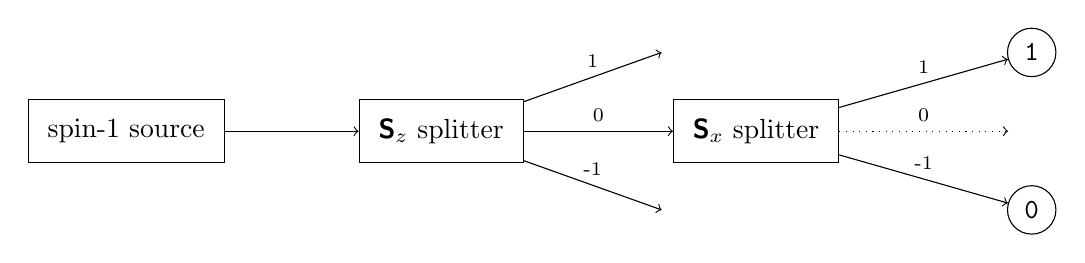
\begin{tikzpicture}
\tikzstyle{c}=[circle,draw,fill=white]
\tikzstyle{r}=[rectangle,draw,fill=white,inner sep=7pt]

\node[r] (source) at (0,0) {spin-1 source};
\node[r] (z) at (4,0) {$\textsf{\textbf{S}}_z$ splitter};
\node[r] (x) at (8,0) {$\textsf{\textbf{S}}_x$ splitter};

\draw[->] (source) -- (z);

\draw[->] (z) edge node[above] {\scriptsize 1} (6.8,1);
\draw[->] (z) edge node[above] {\scriptsize 0} (x);
\draw[->] (z) edge node[above] {\scriptsize -1} (6.8,-1);

\node[c] (1) at (11.5,1) {\texttt{1}};
\node[c] (0) at (11.5,-1) {\texttt{0}};

\draw[->] (x) edge node[above] {\scriptsize 1} (1);
\draw[->,dotted] (x) edge node[above] {\scriptsize 0} (11.2,0);
\draw[->] (x) edge node[above] {\scriptsize -1} (0);
\end{tikzpicture}
\end{center}
\caption{Experimental setup of a configuration of quantum observables rendering random bits certified by quantum value indefiniteness.}
	\label{fig:setup}
\end{figure}


\if01
\begin{table}[h!]
\vspace{-12pt}
\caption{Conflict between $\ket{\textsf{\textbf{S}}_x : 1}$ and $\ket{0}$}
\vspace{-36pt}
\label{tab:1}
$$\begin{array}[t]{|c|c|c|c|c|c|c|c|c|}
\hline
1 & 0 & 1 & 0 & 1 & 0 & 1 & 0 & 1? \\
\hline
\projbf{1}{\sqrt{2}}{1} & \proj{0}{1}{-\sqrt{2}} & \proj{0}{1}{-\sqrt{2}} & \proj{\sqrt{2}}{1}{-\sqrt{2}} & \proj{\sqrt{2}}{1}{-\sqrt{2}} & \proj{\sqrt{8}}{1}{0} & \proj{\sqrt{8}}{1}{0} & \proj{1}{\sqrt{2}}{-1} & \proj{1}{\sqrt{2}}{-1} \\
~ & \proj{\sqrt{2}}{-1}{0} & \proj{1}{0}{0} & ~ & \proj{1}{0}{1} & ~ & \proj{1}{-\sqrt{8}}{3} & ~ & \proj{1}{-\sqrt{2}}{-1} \\
~ & \proj{1}{-\sqrt{8}}{3} & \projbf{0}{\sqrt{2}}{1} & ~ & \projbf{1}{-\sqrt{8}}{-1} & ~ & \projbf{1}{-\sqrt{8}}{-3} & ~ & \proj{1}{0}{1} \\
~ & \proj{1}{-\sqrt{2}}{1} & ~ & ~ & ~ & ~ & ~ & ~ & ~ \\
\projbf{0}{1}{0} & \proj{0}{0}{1} & \proj{0}{0}{1} & \proj{\sqrt{2}}{-1}{-\sqrt{2}} & \proj{\sqrt{2}}{-1}{-\sqrt{2}} & \proj{1}{-\sqrt{2}}{-3} & \proj{1}{-\sqrt{2}}{-3} & \proj{1}{-\sqrt{2}}{-1} & ~ \\
~ & \proj{1}{0}{0} & \proj{\sqrt{2}}{-1}{0} & ~ & \proj{1}{0}{1} & ~ & \proj{1}{-\sqrt{2}}{1} & ~ & ~ \\
~ & \proj{1}{0}{1} & \projbf{1}{\sqrt{2}}{0} & ~ & \projbf{1}{\sqrt{8}}{-1} & ~ & \projbf{\sqrt{2}}{1}{0} & ~ & ~ \\
\hline
\end{array}$$
\vspace{-12pt}
\end{table}

\begin{table}[h!]
\vspace{-12pt}
\caption{Conflict between $\ket{\textsf{\textbf{S}}_x : -1}$ and $\ket{0}$}
\vspace{-36pt}
\label{tab:2}
$$\begin{array}[t]{|c|c|c|c|c|c|c|c|c|}
\hline
1 & 0 & 1 & 0 & 1 & 0 & 1 & 0 & 1? \\
\hline
\projbf{1}{-\sqrt{2}}{1} & \proj{\sqrt{2}}{1}{0} & \proj{\sqrt{2}}{1}{0} & \proj{\sqrt{2}}{1}{-\sqrt{2}} & \proj{\sqrt{2}}{1}{-\sqrt{2}} & \proj{1}{\sqrt{2}}{-3} & \proj{1}{\sqrt{2}}{-3} & \proj{1}{\sqrt{2}}{-1} & \proj{1}{\sqrt{2}}{-1} \\
~ & \proj{0}{1}{\sqrt{2}} & \proj{0}{0}{1} & ~ & \proj{1}{0}{1} & ~ & \proj{1}{\sqrt{2}}{1} & ~ & \proj{1}{-\sqrt{2}}{-1} \\
~ & \proj{1}{\sqrt{2}}{1} & \projbf{1}{-\sqrt{2}}{0} & ~ & \projbf{1}{-\sqrt{8}}{-1} & ~ & \projbf{\sqrt{2}}{-1}{0} & ~ & \proj{1}{0}{1} \\
~ & \proj{1}{\sqrt{8}}{3} & ~ & ~ & ~ & ~ & ~ & ~ & ~ \\
\projbf{0}{1}{0} & \proj{1}{0}{0} & \proj{1}{0}{0} & \proj{\sqrt{2}}{-1}{-\sqrt{2}} & \proj{\sqrt{2}}{-1}{-\sqrt{2}} & \proj{\sqrt{8}}{-1}{0} & \proj{\sqrt{8}}{-1}{0} & \proj{1}{-\sqrt{2}}{-1} & ~ \\
~ & \proj{0}{0}{1} & \proj{0}{1}{\sqrt{2}} & ~ & \proj{1}{0}{1} & ~ & \proj{1}{\sqrt{8}}{3} & ~ & ~ \\
~ & \proj{1}{0}{1} & \projbf{0}{\sqrt{2}}{-1} & ~ & \projbf{1}{\sqrt{8}}{-1} & ~ & \projbf{1}{\sqrt{8}}{-3} & ~ & ~ \\
\hline
\end{array}$$
\vspace{-12pt}
\end{table}





\begin{figure}
\begin{center}
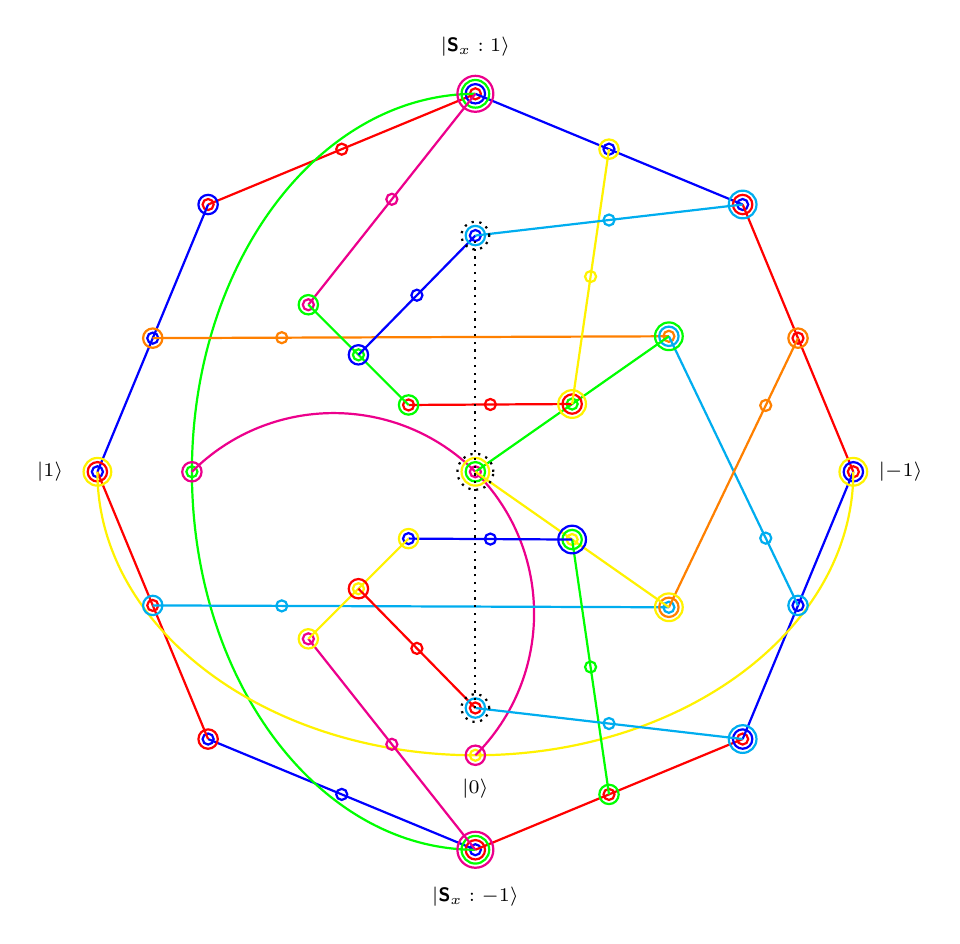
\begin{tikzpicture}[scale=0.6]
\tikzstyle{every path}=[thick]
\tikzstyle{c}=[circle,draw,inner sep=0,minimum size=4]
\tikzstyle{c2}=[circle,draw,inner sep=0,minimum size=7]
\tikzstyle{c3}=[circle,draw,inner sep=0,minimum size=10]
\tikzstyle{c4}=[circle,draw,inner sep=0,minimum size=13]

\draw[red] (90:8) -- (135:8)
	coordinate[c,at start] (1 2 1)
	coordinate[c,midway] (9 -2 -1)
	coordinate[c,at end] (0 1 -2);

\draw[blue] (1 2 1.center) -- (45:8)
	coordinate[c2,at start]
	coordinate[c,midway] (1 2 -9)
	coordinate[c,at end] (2 -1 0);

\draw[blue] (270:8) -- (225:8)
	coordinate[c,at start] (1 -2 1)
	coordinate[c,midway] (9 2 -1)
	coordinate[c,at end] (0 1 2);

\draw[red] (1 -2 1.center) -- (315:8)
	coordinate[c2,at start]
	coordinate[c,midway] (1 -2 -9)
	coordinate[c,at end] (2 1 0);

\draw[green] (90:8) arc (90:270:6 and 8);
	\coordinate[green,c3] (1 2 1) at (90:8);
	\coordinate[green,c] (1 0 -1) at (180:6);
	\coordinate[green,c3] (1 -2 1) at (270:8);

\draw[blue] (180:8) -- (0 1 -2.center)
	coordinate[c,at start] (1 0 0)
	coordinate[c,midway] (0 2 1)
	coordinate[c2,at end];

\draw[red] (1 0 0.center) -- (0 1 2.center)
	coordinate[c2,at start]
	coordinate[c,midway] (0 2 -1)
	coordinate[c2,at end];

\draw[red] (0:8) -- (2 -1 0.center)
	coordinate[c,at start] (0 0 1)
	coordinate[c,midway] (1 2 0)
	coordinate[c2,at end];

\draw[blue] (0 0 1.center) -- (2 1 0.center)
	coordinate[c2,at start]
	coordinate[c,midway] (1 -2 0)
	coordinate[c2,at end];

\draw[yellow] (180:8) arc (180:360:8 and 6);
	\coordinate[yellow,c3] (1 0 0) at (180:8);
	\coordinate[yellow,c] (0 1 0) at (270:6);
	\coordinate[yellow,c3] (0 0 1) at (360:8);

\draw[magenta] (270:6) arc (-45:135:4.24264069);
	\coordinate[magenta,c2] (0 1 0) at (270:6);
	\coordinate[magenta,c] (1 0 1) at (0:0);
	\coordinate[magenta,c2] (1 0 -1) at (180:6);

\draw[orange] (0 2 1.center) -- (35:5)
	coordinate[c2,at start]
	coordinate[c,near start] (9 -2 4)
	coordinate[c,at end] (2 1 -2);

\draw[cyan] (1 -2 0.center) -- (2 1 -2.center)
	coordinate[c2,at start]
	coordinate[c,near start] (4 2 9)
	coordinate[c2,at end];

\draw[cyan] (0 2 -1.center) -- (325:5)
	coordinate[c2,at start]
	coordinate[c,near start] (9 2 4)
	coordinate[c,at end] (2 -1 -2);

\draw[orange] (1 2 0.center) -- (2 -1 -2.center)
	coordinate[c2,at start]
	coordinate[c,near start] (4 -2 9)
	coordinate[c2,at end];

\draw[green] (1 0 1.center) -- (2 1 -2.center)
	coordinate[c2,at start]
	coordinate[c,midway] (1 -8 -1)
	coordinate[c3,at end];

\draw[yellow] (1 0 1.center) -- (2 -1 -2.center)
	coordinate[c3,at start]
	coordinate[c,midway] (1 8 -1)
	coordinate[c3,at end];

\draw[red] (1 -8 -1.center) -- (135:2)
	coordinate[c2,at start]
	coordinate[c,midway] (1 -8 81)
	coordinate[c,at end] (8 1 0);

\draw[yellow] (1 -8 -1.center) -- (1 2 -9.center)
	coordinate[c3,at start]
	coordinate[c,midway] (98 4 18)
	coordinate[c2,at end];

\draw[green] (1 8 -1.center) -- (1 -2 -9.center)
	coordinate[c2,at start]
	coordinate[c,midway] (98 -4 18)
	coordinate[c2,at end];

\draw[blue] (1 8 -1.center) -- (225:2)
	coordinate[c3,at start]
	coordinate[c,midway] (1 8 81)
	coordinate[c,at end] (8 -1 0);

\draw[magenta] (1 2 1.center) -- (135:5)
	coordinate[c4,at start]
	coordinate[c,midway] (50 -4 -18)
	coordinate[c,at end] (1 -8 9);

\draw[magenta] (1 -2 1.center) -- (225:5)
	coordinate[c4,at start]
	coordinate[c,midway] (50 4 -18)
	coordinate[c,at end] (1 8 9);

\draw[green] (1 -8 9.center) -- (8 1 0.center)
	coordinate[c2,at start]
	coordinate[c,midway] (1 -8 -9)
	coordinate[c2,at end];

\draw[yellow] (1 8 9.center) -- (8 -1 0.center)
	coordinate[c2,at start]
	coordinate[c,midway] (1 8 -9)
	coordinate[c2,at end];

\draw[blue] (1 -8 -9.center) -- (90:5)
	coordinate[c2,at start]
	coordinate[c,midway] (50 -4 18)
	coordinate[c,at end] (1 2 -1);

\draw[red] (1 8 -9.center) -- (270:5)
	coordinate[c2,at start]
	coordinate[c,midway] (50 4 18)
	coordinate[c,at end] (1 -2 -1);

\draw[cyan] (2 1 0.center) -- (1 -2 -1.center)
	coordinate[c3,at start]
	coordinate[c,midway] (1 -2 9)
	coordinate[c2,at end];

\draw[cyan] (2 -1 0.center) -- (1 2 -1.center)
	coordinate[c3,at start]
	coordinate[c,midway] (1 2 9)
	coordinate[c2,at end];

\draw[dotted] (1 -2 -1.center) -- (1 2 -1.center)
	coordinate[c3,at start]
	coordinate[c4,midway]
	coordinate[c3,at end];

\node at (90:9) {\scriptsize $\ket{\textsf{\textbf{S}}_x : 1}$};
\node at (270:9) {\scriptsize $\ket{\textsf{\textbf{S}}_x : -1}$};
\node at (0:9) {\scriptsize $\ket{-1}$};
\node at (180:9) {\scriptsize $\ket{1}$};
\node at (270:6.7) {\scriptsize $\ket{0}$};
\end{tikzpicture}
\end{center}
\caption{Orthogonality diagram of a configuration of quantum observables rendering a proof that certain random bits are certified by quantum value indefiniteness.}
\label{fig:greechie}
\end{figure}
\fi

\subsection{Certification via value indefiniteness}

Consider the QRNG
%\footnote{We consider a QRNG, as proposed in \cite{}, which for example repeatedly prepares the system in an eigenstate of an observable $A$ and measures the result of an observable $B$ satisfying $[A,B]\neq 0$.}
described in the previous section, and let us consider that we run it repeatedly `to infinity'---i.e. we use it repeatedly to generate bits and concatenate them together to produce, in the limit, the binary sequence $\seq{x}=x_1 x_2 \dots x_n \dots$.
Here we consider the sequence $\seq{x}$ produced in such a manner and show that, under our assumptions, it is guaranteed to be incomputable.
Note that we are using the Measurement Assumption here, since we must assume that $\seq{x}$ is actually produce (not that, e.g., all infinite sequences are generated in different universes).

Let us assume for the sake of contradiction that $\seq{x}$ as described above is computable.
Then, by definition, there must exist a Turing machine $T$ (and thus a computable function) that can be associated with $\seq{x}$ allowing us to predict with certainty every value $x_i$.
From the E.p.r. assumption, it follows that each observable $o_i$ is value definite and $v_i(o_i,C)=x_i$.
But, by our QRNG design, the observable $o_i$ is at an angle $\pi/4$ with the observable which the state is prepared in, and, since the preparation context must be value definite (by the eigenstate assumption), from Theorem~\ref{thm:twonotvaluedefinite} we have that $v_i(o_i,C)$ is not defined, a contradiction.
Thus we conclude that $\seq{x}$ must be incomputable.

This proof can easily show the stronger claim: that $\seq{x}$ is bi-immune (no infinite sub-sequence of $\seq{x}$ is computable).
This can easily by seen by the same argument: if there was a computable subsequence then we could assign definite values to the observables giving rise to this subsequence, contradicting our assumption of value indefiniteness everywhere.


%From the ternary sequence $\seq{x}$ we effectively compute the binary sequence $\seq{y}= y_{1}y_{2} \dots y_{m}\dots $ such that
%$\sum_{n=1}^{\infty} x_{n}  3^{-n}= \sum_{m=1}^{\infty} y_{n} 2^{-m}$, and conversely. If follows that the bi-immunity of $\seq{x}$
%implies bi-immunity of $\seq{y}$ too.

We have proved:\\

\begin{Theorem} Assume Non-contextuality, Measurement, Eigenstate and E.p.r. assumptions.  Then there exits a QRNG which generates a bi-immune binary sequence.
\end{Theorem}

We further note that this result is more general than that proved in \cite{} and does not require any assumption about the uniformity of bits produced.



\section{Realisation in terms of generalised beam splitters}
\label{sec:experiment}

In this section we describe a realisation of the QRNG described in the previous section.
Since it is not particularly feasible to directly use spin-1 particles [?] in a QRNG with an acceptably high bit-rate, the realisation we present uses photons and is in terms of generalised beam-splitters.\marginpar{details?}

Consider an orthonormal cartesian standard basis
$\vert 1\rangle \equiv (1,0,0)$,
$\vert 0\rangle \equiv  (0,1,0)$, and
$\vert -1\rangle \equiv  (0,0,1)$.
Then, in order to realize observables such as the spin state observables
\begin{equation}
\textsf{\textbf{S}}(\theta,\phi )
=
\left(
\begin{array}{ccc}
 \cos (\theta ) & \frac{e^{-i \phi } \sin (\theta )}{\sqrt{2}} & 0 \\
 \frac{e^{i \phi } \sin (\theta )}{\sqrt{2}} & 0 & \frac{e^{-i \phi } \sin (\theta )}{\sqrt{2}} \\
 0 & \frac{e^{i \phi } \sin (\theta )}{\sqrt{2}} & -\cos (\theta )
\end{array}
\right);
\end{equation}
and, in particular, spin states  measured along the $x$-axis;
that is, for $\theta = \frac{\pi}{2}$ and $\phi = 0$,
\begin{equation}
\textsf{\textbf{S}}_x   =
\textsf{\textbf{S}}(\frac{\pi}{2},0 )
=
\left(
\begin{array}{ccc}
 0 & \frac{1}{\sqrt{2}} & 0 \\
 \frac{1}{\sqrt{2}} & 0 & \frac{1}{\sqrt{2}} \\
 0 & \frac{1}{\sqrt{2}} & 0
\end{array}
\right)
\end{equation}
in terms of generalized beam splitters, the
associated normalized row eigenvectors
\begin{equation}
\begin{array}{l}
 \vert \textsf{\textbf{S}}_x : +1 \rangle \equiv  \left(1,\sqrt{2},1\right),\\
 \vert \textsf{\textbf{S}}_x : 0 \rangle \equiv  \left(1,0,-1\right),\\
 \vert \textsf{\textbf{S}}_x : -1 \rangle \equiv  \left(1,-\sqrt{2},1\right)
\end{array}
\end{equation}
have to be ``stacked'' on top of one another \cite{rzbb}, thereby forming a unitary matrix $\textsf{\textbf{U}}_x $
which correspond to the spin state operator $\textsf{\textbf{S}}_x$ for spin state measurements along the $x$-axis;
more explicitly,
\begin{equation}
\textsf{\textbf{U}}_x
=
\frac{1}{2}
\left(
\begin{array}{cccc}
1&\sqrt{2}&1\\
\sqrt{2}&0&-\sqrt{2}\\
1&-\sqrt{2}&1
\end{array}
\right).
\end{equation}

The physical realization of $\textsf{\textbf{U}}_x$ is depicted in Fig.~\ref{2012-incomput-proofsC-f1}.

\begin{figure}[ht]
\begin{center}

%TexCad Options
%\grade{\off}
%\emlines{\off}
%\beziermacro{\on}
%\reduce{\on}
%\snapping{\off}
%\quality{2.00}
%\graddiff{0.01}
%\snapasp{1}
%\zoom{10.00}
\unitlength 20mm
\linethickness{0.8pt}
\begin{picture}(6,5)(-3.0,-1.5)

\put(-2.6,3){\line(0,-1){3}}

\put(-2.6,2.5){\line(1,1){0.2}}
\put(-2.6,2.5){\line(-1,1){0.2}}

\put(-2.6,2){\line(1,0){1}}
\put(-2.6,1){\line(1,0){1}}
\put(-2.6,0){\line(1,0){1}}

\put(-1.6,2){\line(-1,1){0.2}}
\put(-1.6,2){\line(-1,-1){0.2}}
%\put(-2.6,2){\color{green} \oval(0.14,0.14)[rt]}
%\put(-2.47,2.12){\makebox(0,0)[cc]{\color{green} \tiny $\varphi$}}
%\put(-2.8,2.2){\color{green} \line(1,-1){0.4}}
%\put(-2.8,1.8){\color{green} \framebox(0.4,0.4)[cc]{}}
 \put(-2.4,2.3){\makebox(0,0)[lc]{\color{green} $T=1$}}
%\put(-2.4,1.6){\makebox(0,0)[lc]{\color{green} $T=\frac{2}{3}$}}
% \put(-2.2,1.9){\color{blue} \rule{0.4cm}{0.4cm} }
% \put(-2.2,2.25){\makebox(0,0)[lc]{\color{blue}$-\varphi$}}

\put(-1.6,1){\line(-1,1){0.2}}
\put(-1.6,1){\line(-1,-1){0.2}}
\put(-2.6,1){\color{green} \oval(0.14,0.14)[rt]}
%\put(-2.47,1.12){\makebox(0,0)[cc]{\color{green} \tiny $\frac{\pi}{2}$}}
\put(-2.47,1.12){\makebox(0,0)[cc]{\color{green} \tiny $ \pi $}}
\put(-2.8,1.2){\thicklines \color{green} \line(1,-1){0.4}}
\put(-2.8,0.8){\color{green} \framebox(0.4,0.4)[cc]{}}
\put(-2.4,0.6){\makebox(0,0)[lc]{\color{green} $T= 0 $}}
%\put(-2.4,0.6){\makebox(0,0)[lc]{\color{green} $T=\frac{1}{2}$}}
 \put(-2.2,0.9){\color{blue} \rule{0.4cm}{0.4cm} }
% \put(-2.2,1.25){\makebox(0,0)[lc]{\color{blue}$-\frac{\pi}{2}$}}
 \put(-2.2,1.25){\makebox(0,0)[lc]{\color{blue}$- \pi $}}

\put(-1.6,0){\line(-1,1){0.2}}
\put(-1.6,0){\line(-1,-1){0.2}}

\put(-1.2,1.7){\color{brown} \rule{0.2cm}{1.2cm} }
\put(-1.2,-0.3){\color{brown} \rule{0.2cm}{1.2cm} }

\put(1.22,1.3){\makebox(0,0)[lc]{\color{green} $T=1$}}
\put(0.5,1){\line(1,0){1.00}}
\put(1,0.5){\line(0,1){1.00}}
%\put(0.9,0.5){\framebox(0.2,0.05)[cc]{}}
%\put(1.2,0.55){\makebox(0,0)[lc]{$0$}}
%\put(0.9,0.5){\color{blue}\framebox(0.2,0.05)[cc]{}}
%\put(0.9,0.5){\color{blue} \rule{0.4cm}{0.4cm} }
%\put(1.2,0.55){\makebox(0,0)[lc]{\color{blue}$-\frac{\pi}{2}$}}
\put(0.5,0){\line(1,0){1.00}}
\put(1,-0.5){\line(0,1){1.00}}
\put(1.5,0){\line(1,0){1.00}}
\put(2,-0.5){\line(0,1){1.00}}
\put(0,2){\line(1,0){0.50}}
\put(-0.48,2){\makebox(0,0)[cc]{$\vert \textsf{\textbf{S}}_z : -1 \rangle$}}
\put(3,-0.5){\line(0,-1){0.50}}
\put(3,-1){\line(1,1){0.2}}
\put(3,-1){\line(-1,1){0.2}}
\put(3,-1.2){\makebox(0,0)[cc]{$\vert \textsf{\textbf{S}}_x : -1 \rangle$}}
\put(0.5,2){\line(1,0){0.5}}
\put(1,2){\line(0,-1){0.5}}
\put(0,1){\line(1,0){0.50}}
\put(-0.48,1){\makebox(0,0)[cc]{$\vert \textsf{\textbf{S}}_z : 0 \rangle$}}
\put(2,-0.5){\line(0,-1){0.50}}
\put(2,-1){\line(1,1){0.2}}
\put(2,-1){\line(-1,1){0.2}}
\put(2,-1.2){\makebox(0,0)[cc]{$\vert \textsf{\textbf{S}}_x : +1 \rangle$}}
\put(1.5,1){\line(1,0){0.5}}
\put(2,1){\line(0,-1){0.5}}
\put(0,0){\line(1,0){0.50}}
\put(-0.48,0){\makebox(0,0)[cc]{$\vert \textsf{\textbf{S}}_z : +1 \rangle$}}
\put(1,-0.5){\line(0,-1){0.50}}
\put(1,-1){\line(1,1){0.2}}
\put(1,-1){\line(-1,1){0.2}}
\put(1,-1.2){\makebox(0,0)[cc]{$\vert \textsf{\textbf{S}}_x : 0 \rangle$}}
\put(2.5,0){\line(1,0){0.5}}
\put(3,0){\line(0,-1){0.5}}
\put(1.22,0.3){\makebox(0,0)[lc]{\color{green} $T=\frac{1}{2}$}}
\put(1,0){\color{green} \oval(0.14,0.14)[rt]}
\put(1.13,0.12){\color{green} \makebox(0,0)[cc]{\tiny $\frac{\pi}{2}$}}
\put(0.8,0.2){\color{green} \line(1,-1){0.4}}
\put(0.8,-0.2){\color{green} \framebox(0.4,0.4)[cc]{}}
\put(2.22,0.3){\makebox(0,0)[lc]{\color{green} $T=\frac{1}{2}$}}
\put(2,0){\color{green} \oval(0.14,0.14)[rt]}
\put(2.13,0.12){\makebox(0,0)[cc]{\color{green} \tiny $\frac{\pi}{2}$}}
\put(1.8,0.2){\color{green} \line(1,-1){0.4}}
\put(1.8,-0.2){\color{green} \framebox(0.4,0.4)[cc]{}}
 \put(1.9,0.5){\color{blue} \rule{0.4cm}{0.4cm} }
 \put(2.2,0.55){\makebox(0,0)[lc]{\color{blue}$ \frac{\pi}{2}$}}
 \put(0.9,1.5){\color{blue} \rule{0.4cm}{0.4cm} }
 \put(1.2,1.55){\makebox(0,0)[lc]{\color{blue}$-\frac{\pi}{2}$}}
 \put(0.9,-0.5){\color{blue} \rule{0.4cm}{0.4cm} }
 \put(1.2,-0.45){\makebox(0,0)[lc]{\color{blue}$-\frac{\pi}{2}$}}
 \put(1.9,-0.5){\color{blue} \rule{0.4cm}{0.4cm} }
 \put(2.2,-0.45){\makebox(0,0)[lc]{\color{blue}$-\frac{\pi}{2}$}}
%\put(2.9,-0.5){\framebox(0.2,0.05)[cc]{}}
%\put(3.2,-0.45){\makebox(0,0)[lc]{$0$}}
\end{picture}
\end{center}
\caption{(Color online) Configuration of a random number generator
with a preparation and a measurement stage, including filters blocking
$\vert \textsf{\textbf{S}}_z : -1 \rangle$
and
$\vert \textsf{\textbf{S}}_z : +1 \rangle$.
(For ideal beam splitters, these filters would not be required.)
The measurement stage (right array) realizes a unitary quantum gate $\textsf{\textbf{U}}_x$, corresponding  to the projectors onto
the $\textsf{\textbf{S}}_x$ state observables for spin state measurements along the $x$-axis,
in terms of generalized beam splitters.
\label{2012-incomput-proofsC-f1}}
\end{figure}

An inspection of the generalized beam splitter setup reveals that it actually consists of a standard 50:50 beam splitter device
used for quantum coin tosses
\cite{svozil-qct,rarity-94,zeilinger:qct,stefanov-2000,0256-307X-21-10-027,wang:056107,fiorentino:032334,svozil-2009-howto,10.1038/nature09008},
with the addition of additional optical components remaining ``idle'' or ``dormant''
in the case of ideal components.
This is due to the effectively quasi two-dimensionality of the dichotomic outcome setup,
which may be not so evident in the case of spin state measurements on spin one particles.
However, one should keep in mind that
the device is capable of performing transformations and rendering observables in full three dimensional Hilbert space,
with all the counterfactual potentialities present.
This in a sense, is not dissimilar to counterfactual computation  \cite{elitzur-vaidman:1}.


\section{Monitoring value indefiniteness}

The rendition of value indefiniteness requires a quantised system with at least three mutually exclusive outcomes,
corresponding to an associated Hilbert space dimension equal to the number of these outcomes.
This is a direct consequence of the Kochen-Specker theorem; as well as related \cite{PhysRevLett.103.050401} or unrelated \cite{Pit-94}
Bell-type inequalities representing classical bounds on joint probabilities.
The Kochen-Specker theorem, in turn, is obtained by a proof by contradiction (or {\it ``reductio ad absurdum''}),
which appears to be a finite, constructive formal argument from a metamathematical point of view.

Of course, if one is willing to accept physical value indefiniteness
based purely on formal  Hilbert space models of quantum mechanics \cite{v-neumann-55},
there is no further need of empirical evidence.
In this line of thinking, the Kochen-Specker theorem, and hence quantum value indefiniteness resulting from it, needs no more empirical corroboration
than the arithmetic fact that, with the assumption of Peano arithmetic and standard addition, one plus one equals two.

Nevertheless, given the highly nontrivial assumptions entering the Kochen-Specker theorem -- in particular, the mutual physical coexistence of
complementary observables --
it might be considered more appropriate to at least possess some indication, hints or limited certifications relating the nonclassical features
of these types of arguments with empirical findings; even if these findings do not constitute a proof
in the strict meaning of the term.

There are some indirectly obtained physical remedies which are often referred to as
``proofs of the Kochen-Specker theorem,''
or to ``proofs of quantum contextuality''
\cite{hasegawa:230401,Bartosik-09,kirch-09,PhysRevLett.103.160405,Lapkiewicz-11}.
Thus if one is
willing to either accept as proofs certain Bell type arguments about a series of successive (``one-after-another'') outcomes \cite{PhysRevLett.103.160405},
or to accept the type of nonclassical outcomes typically encountered in
empirical realizations of Greenberger-Horne-Zeilinger type arguments \cite{PhysRevLett.82.1345,panbdwz},
then indeed value indefiniteness or contextuality are physically provable.

With this {\it caveat} we propose to {\em monitor} all protocols invoking value indefiniteness or contextuality by
physical experiments testing the nonclassical nature of the quantized systems involved.
This could be either achieved by invoking the aforementioned violations of Bell-type inequalities \cite{10.1038/nature09008}, or by
experiments invoking  Greenberger-Horne-Zeilinger type measurements.
The latter ones may be preferable, since, at least ideally, they do not involve any statistics,
but require a violation of local realism at every triple of outcomes.
Of course, in order to monitor this nonclassical behaviour, protocols must be adapted to
include such measurements involving multipartite correlations.


In the concrete beam splitter configutation mentioned earlier one could monitor the nonclassicality of the setup
by first producing the (only \cite{schimpf-svozil}) singlet state
$\frac{1}{{\sqrt{3}}}\left(-|0,0\rangle+|-1,1\rangle+|1,-1\rangle\right)$,
and then subjecting the two entangled quanta to beam splitter analysis.
We refer to Refs.~\cite{zukowski-97} and \cite{svozil-2004-analog} for two principal approaches.
The Bell-type inequalities violated in this case are the two particle  three properties per particle
inequalities derived in Refs.~\cite{2000-poly,collins-gisin-2003,sliwa-2003}.

\bibliographystyle{plain}
\bibliography{svozil.bib}%,alastairBib,alastairBib.bib,hypercomputation.bib}


\end{document}
